% Source note: notes/2026-10-19-mt2-solo-publication-talk.md
\begin{entry}{research}{2026-10-19}{MT2 SOLO paper: 3 min presentation}
\entrytags{aad, motivation}

Source: handwritten notes (2 pages), transcribed

Task: set in MT1 (choose a DIMT publication via SOLO), presented as a 3-min talk in MT2.

Reference: \fullcite{Bellier2023}
\nocite{Bellier2023}

\subsection*{1) What it is}
Pink Floyd

29 epilepsy patients, already implanted with electrodes for clinical reasons, listened to Pink Floyd's Another Brick in the Wall. The team reconstructed the song's spectrogram from that activity, and the output was recognisable.

\subsection*{2) The problem}
Prosody vs content

Trying to work out which brain regions handle which musical tones, rhythms etc.\ in the context of a naturalistic song rather than isolated tones. Speech BCIs sound robotic because we don't know how to decode prosody, even if we can decode words. Music is a model for the expression.

\subsection*{3) What's novel?}
First reconstruction of a song, rather than just classification.

Non-linear neural network approach beats the linear: $r^2$ 0.429 vs 0.325, 32\% gain, and only the non-linear version was recognisable.

Both saturate fast, 80\% of accuracy could be obtained with just 43 of 347 electrodes, or 37 seconds of the song.

Detected part of the mid-STG brain region, locked on to the beat of the music.

\subsection*{4) Who?}
Bellier and Knight: UC Berkeley's Helen Wills Neuroscience Institute, biomedical engineering at Florida, neurology at Albany Medical College, neurosurgery at Washington University Neuroscience \& Medicine.

\subsection*{5/6) Product \& user}
A speech neuroprosthesis that preserves prosody, so a synthesised voice carries emphasis and emotion rather than sounding flat. Users: people with ALS, locked-in syndrome, or anarthria after a brainstem stroke. The 43 electrode result is achievable, much easier to create a device.

\subsection*{What it means for us}
\begin{itemize}
  \item They perceived the song, they didn't imagine it.
  \item Consumer EEGs can't detect the high frequencies we need and the skull acts as a low pass filter.
  \item But the parts of the spectrogram relating to rhythm, beat, structural stems, were low frequencies, so it might be possible to reconstruct rhythm at the least.
\end{itemize}

\begin{figure}[htbp]
  \centering
  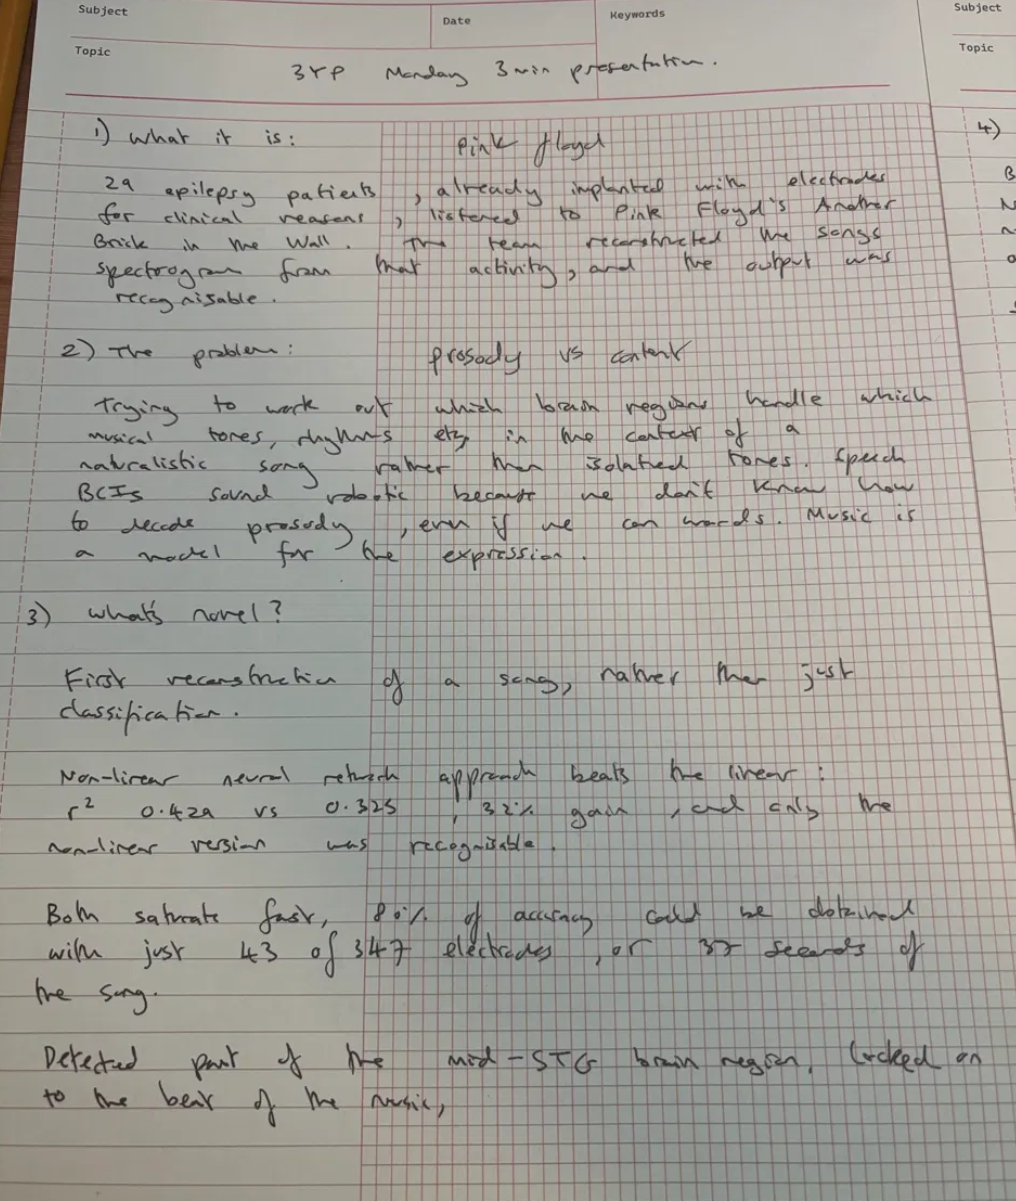
\includegraphics[width=0.48\textwidth]{2026-10-19-mt2-notes-p1.png}\hfill
  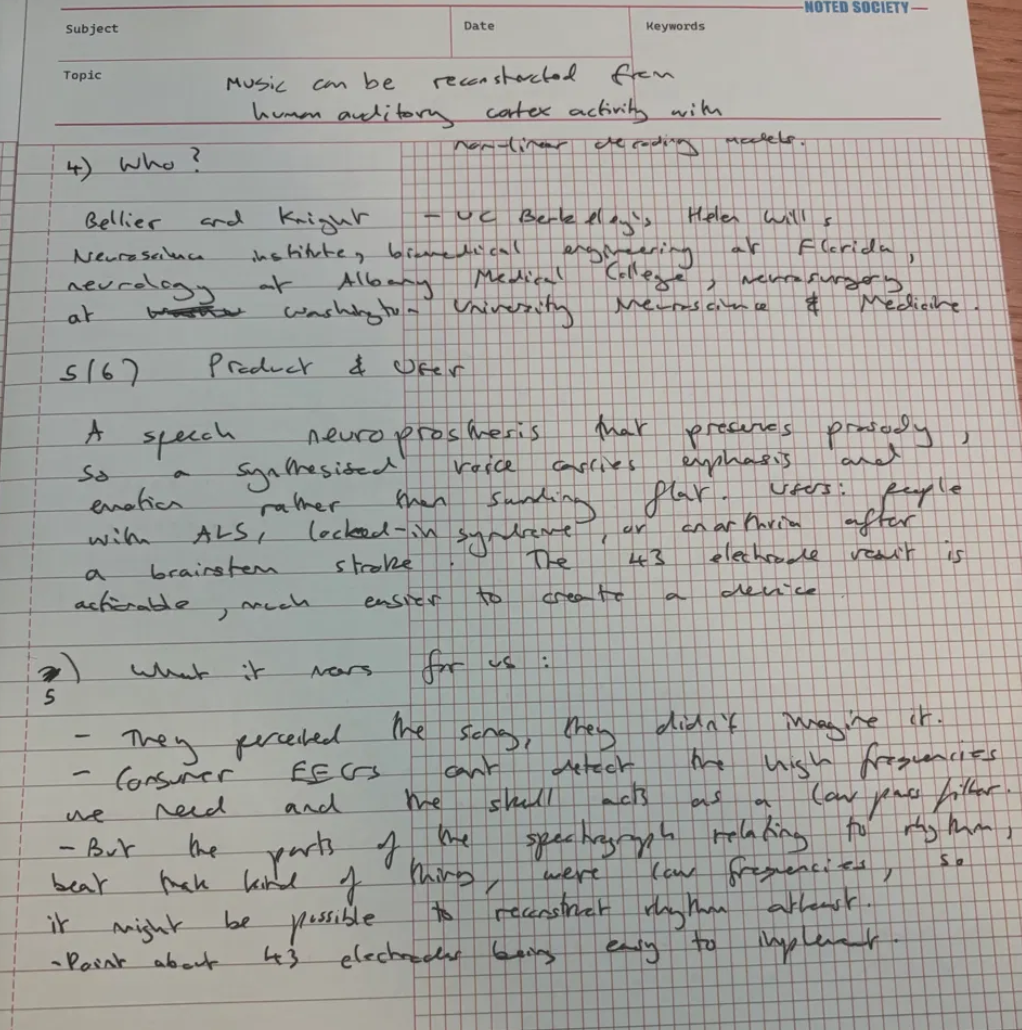
\includegraphics[width=0.48\textwidth]{2026-10-19-mt2-notes-p2.png}
  \caption{Handwritten original notes, pages 1 and 2.}
\end{figure}
\end{entry}
